\section{单频波的程序}
我们将按他的启示行事。你的第一个问题与图\ref{lst:code2.3.1}所示之计算机程序有关。照实际情形来说,它将产生通过某一能量的波动传播的活动电影
(三维矩阵形式)。从编辑到计算直至最终看见循环影片的整个过程,约为一分钟(当你是计算机仅有的用户的时候)。
\subsection{循环影片程序之分析}
要使循环影片对观众有意义,电影的主题必须是周期性的,从而必须安排得使最后的
面很自然地与第一个画面衔接起来。在图\ref{lst:code2.3.1}所示程序形成的电影中,有一个参量
lambda,它控制着从顶部照亮屏幕之波动脉冲的基本重复率。当一个子波往下传播了四分
之一画面的路程时,另一个子波就应送进去。这种过程由下列一行程序来规定
\begin{equation*}
lambda=nz*dz/4=\frac{N_z\Delta_z}{4}
\end{equation*}
各脉冲均由频率为$n\omega$、即$\Delta \omega$、$2\Delta\omega\ldots\ldots$,$n\omega\Delta\omega$等之正弦波叠加而形成,最低频率$d\omega=\Delta\omega$
具有与lambda呈反比的波长。因此规定
\begin{equation*}
d\omega=v\times\pi^2/lambda=\frac{2\pi v}{\lambda}
\end{equation*}
最后,循环影片的延续时间必须等于最低频正弦波的周期
\begin{equation*}
N_t\Delta t=\frac{2\pi}{\Delta \omega}
\end{equation*}
最后这个方程定义了关于扫描线的时间间隔
\begin{equation*}
dt=\pi^2/(nt\times d\omega)
\end{equation*}
该程序所求解的偏微分方程为
\begin{equation}
\frac{\partial P}{\partial z}=\frac{i\omega}{v(x,z)}P+\frac{v}{-i\omega^2}\frac{\partial^2 P}{\partial x^2}
\label{eq:ex2.3.1}
\end{equation}
对于每个步长$\Delta z$,完成两步计算,第一步是解
\begin{equation}
\frac{\partial Q}{\partial z}=\frac{v}{-i\omega^2}\frac{\partial^2 Q}{\partial x^2}
\label{eq:ex2.3.2}
\end{equation}
利用Crank-Nicolson差分方法,此式变为
\begin{equation*}
\frac{q_{z+1}^x-q_z^x}{\Delta z}=-\frac{v}{i\omega^2}[\frac{q_z^{x+1}-2q_z^x+q_z^{x-1}}{2\Delta x^2}+
\frac{q_z^{x+1}-2q_{z+1}^x+q_{z+1}^{x-1}}{2\Delta x^2}]
\end{equation*}
将所有常数减缩成一个常数,并定义:
\begin{equation}
\alpha=\frac{v\Delta z}{-i\omega^4\Delta x^2}
\label{eq:ex2.3.3}
\end{equation}
得到
\begin{equation*}
q_{z+1}^x-q_z^x=\alpha[q_z^{x+1}-2q_z^x+q_z^{x-1}+q_z^{x+1}-2q_{z+1}^x+q_{z+1}^{x-1}]
\end{equation*}
将各未知数置于左端,则
\begin{equation}
-\alpha q_{z+1}^{x+1}+(1+2\alpha)q_{z+1}^x-\alpha q_{z+1}^{x-1}=\alpha q_z^{x+1}+(1-2\alpha)q_z^x+
\alpha q_z^{x-1}
\label{eq:ex2.3.4}
\end{equation}
第二步是解下述方程
\begin{equation}
\frac{\partial Q}{\partial z}=\frac{i\omega}{v}Q
\label{eq:ex2.3.5}
\end{equation}
其解析解为
\begin{equation}
Q(z+\Delta z)=Q(z)e^{i\frac{\omega}{v}\Delta z}
\label{eq:ex2.3.6}
\end{equation}
图\ref{lst:code2.3.1}中的程序严格按\ref{eq:ex2.3.3}、\ref{eq:ex2.3.4}与\ref{eq:ex2.3.6}各式而编制。
\begin{listing}[H]
  \caption{产生单频波之和的电影的计算机程序}
  \inputminted{Fortran}{timespace/code2-3-1.f90}
  \label{lst:code2.3.1}
\end{listing}
\subsection{相移}
为作出波动脉冲,须将若干频率成分相加起来。在这个程序中,只利用了两个频率
$nw=2$。如果你试图只用一个频率$nw =1$
,则有些事情就变得不太清晰了。在侧边界上反射
回来的波看起来更像是驻波(参考练习2)。如果你试图采用更多频率,程序就将比较长了,
但是你会更喜欢那画面,因为脉冲之间的平静区会比较长而平静一些。各种频率成分可采用
不同的加权。
%\begin{minted}{Fortran}
%# submit
%nx = 13
%\label{prog:2.3.1}
%\end{minted}

% \begin{figure}[H]
% \centering
% 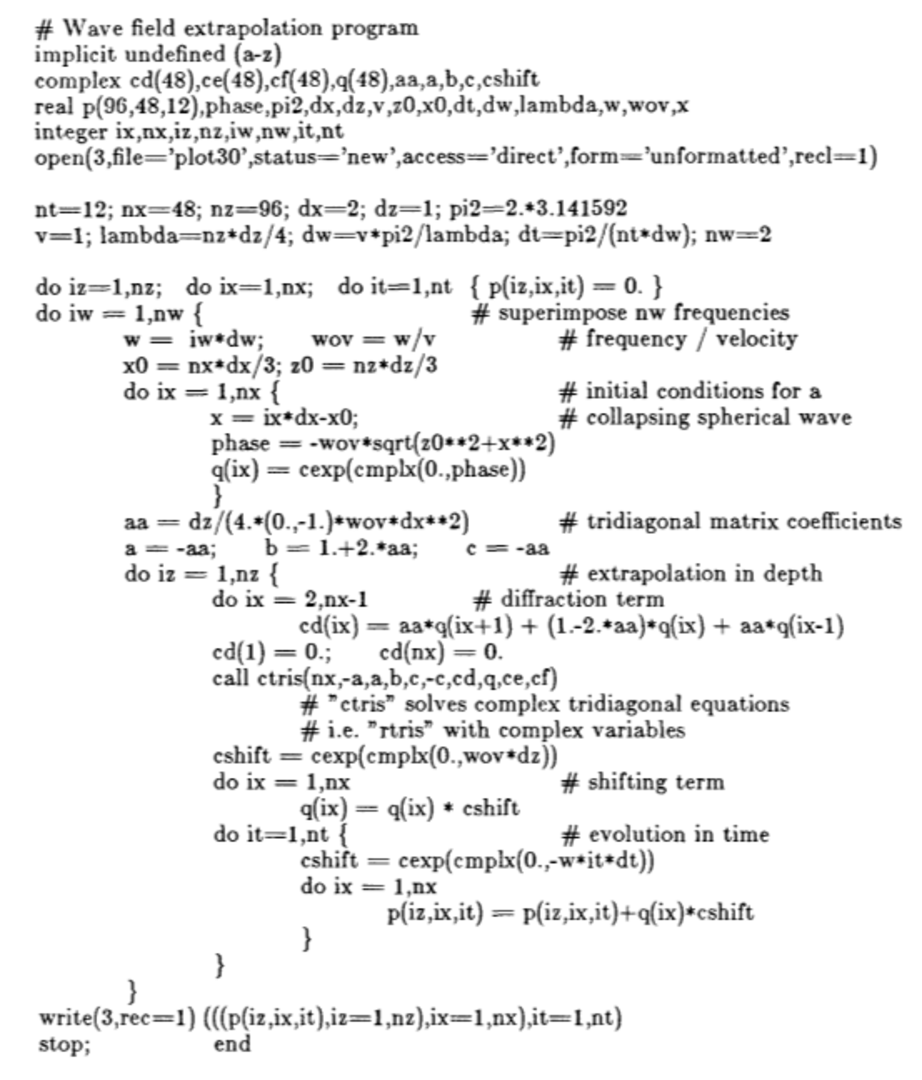
\includegraphics[width=0.85\textwidth]{new/fig-2-3-1}
% \caption[code2-3-1]{产生单频波之和的电影的计算机程序}
% \label{fig:new/fig-2-3-1}
% \end{figure}
理论预言,经过一焦点的二维波动将经受90°的相移。你应能注意到,一个对称波形入
射在焦点上,但是却形成了一个反对称的波形。(在图\ref{fig:2.3.6}中可以很好地看出这点,但在电影
中比较清楚)。在地震偏移方法中,波是正好到达焦点而不是通过它,所以二维情形的偏移脉
冲响应有45°相移。尽管现实世界是三维的,对于推测是由柱面而非球面反射面引起聚焦之
处的地震测线,适宜于进行偏移的却是二维响应。

\subsection{横向速度变化}
横向速度变化$v=v(x)$尚未包括在程序之中,不过把它加进去并不困难。它从两个地
方进入程序,第一是进入式\ref{eq:ex2.3.6},如果$k_x$是足够小以致可忽略不计的数据,则式
\ref{eq:ex2.3.6}就是仅有的需要该项速度之处。第二是进入三对角线系数。光学上的所谓薄透镜
近似看来好像仅只相当于包括式\ref{eq:ex2.3.6}这一部分。

\subsection{侧边界分析}
在地球物理学中,我们通常都希望别同侧边界问题沾边。要考虑侧边界问题的唯一实际
原因是我们的勘测或者我们的处理活动有必要对其范围加以限制。既然侧边界是不可避免
的,那我们就必须想办法对付它。\ref{lst:code2.3.1}内的程序包括有零斜率边界条件,取
\begin{equation*}
d(1)=0.; d(nx)=0.
\end{equation*}
并在调用子程序“ctris”时取
\begin{equation*}
endl= -a ; endr = -c
\end{equation*}
即可形成此类边界条件。得到零值侧边界条件的快速方法是取
\begin{equation*}
endl = endr = 10^{30}\approx\infty
\end{equation*}
上述处理办法稍微有点浪费计算机内存,因为端点的零值要存储起来,而零斜率则可明
显看成是有两个相同的记录道,Dave
Hale所编制的程序可避免这种浪费,该程序给出如下:
\begin{minted}{Fortran}
qO = bl * q ( 1 ) ; qnxpl=br * q ( nx )

cd ( 1 ) = aa * q ( 2 ) + (1.-2. * aa ) * q ( 1 ) +aa * qO
cd ( nx ) =aa * q ( nx-1 ) + ( 1.-2. * aa ) * q ( nx )+aa * qnxpl

endl=c * bl + b;
endr=a * br + b

call ctris (nx, endl, a, b, c, endr, cd, q, ce, cf)
\end{minted}
注意,对于零值边界应$bl=br=0$,对于零斜率边界则应$bl=br=
l$。令bl与br为复数,则可得到\ref{sec:4.4}节中将导出的吸收边界条件。

\subsection{关于循环影片程序的若干变种}
通过以下的一些练习来记录你的进步,在准备期终考试时,这将是有帮助的。而且此后
若干年你都能重温你的记忆。

准备一本活页笔记簿,把所有图件和程序纸裁成长11宽$8\frac{1}{2}$大小,并穿三个孔。若需要
进行代数分析,那就在另一张同样大小的纸上作,别把重要一点的分析写在碎纸片上。这份
材料同你的课堂笔记一起保留,或者作为一本实验笔记簿保存。始终别忘填上日期。

对这些练习的每一个题,均须送交一份程序和第一个画面的图。

练习1试说明如何改变程序,使之得出一个右侧偏离垂直线呈15°角度向下传播的初始
平面波。

练习2已知计算域为$0<x\leq x_{max}$和$0<z\leq z_{max}$,你将如何更改$z=0$处的初始条件,使
之可模拟一在$(x,z) =(x_{max}/3,-z_{max}/2)$处的点源?

练习3试修改程序,使得可用零偉侧边界来代替零斜率边界。

练习4试对衰减球面波应用45°项$\partial _{xxz}$。利用零斜率边界。将你所得结果同用图\ref{lst:code2.3.1}的
程序所得结果进行比较。在理论焦点位置上作一记号$X$。

练习5对程序进行一些改变,使之包括一个薄透镜项,通过恒定慢度梯度所产生的画
面时该透镜项具有40\%的横向速度变化.识别出程序中为横向速度变化所影响的其他部分。
你无需去进行其他这些改变。试问为何预计这些变化会很小?

练习6试利用位于$(x,z)=(x_{max}/2,0)$的一个点震源来检验程序,请观察并描
绘出各种计算产生的假象。这类震源富含很高空间频率,在这种情况下,差分方程无法模拟
其相应的微分方程。

练习7 \ref{sec:4.4}节将阐述如何在侧边界上使能量被吸收。试按此要求对程序作必要的改 变。

练习8采用以后在\ref{sec:4.3}
节述及的方法能够改善$x$方向的导数之精度。主要之点是,不用
主对角线元素为$(-1,2,-1)$的三对角线矩阵$\mathbf{T}$来代表$k_x^2\Delta x^2$,而是用$\mathbf{T}/(\mathbf{I}-\mathbf{T}/6)$。因
遍乘以该分母而须修改原来的外推分析方法。试对45°衰减波的程序进行必要的改变。
\begin{figure}[H]
\centering
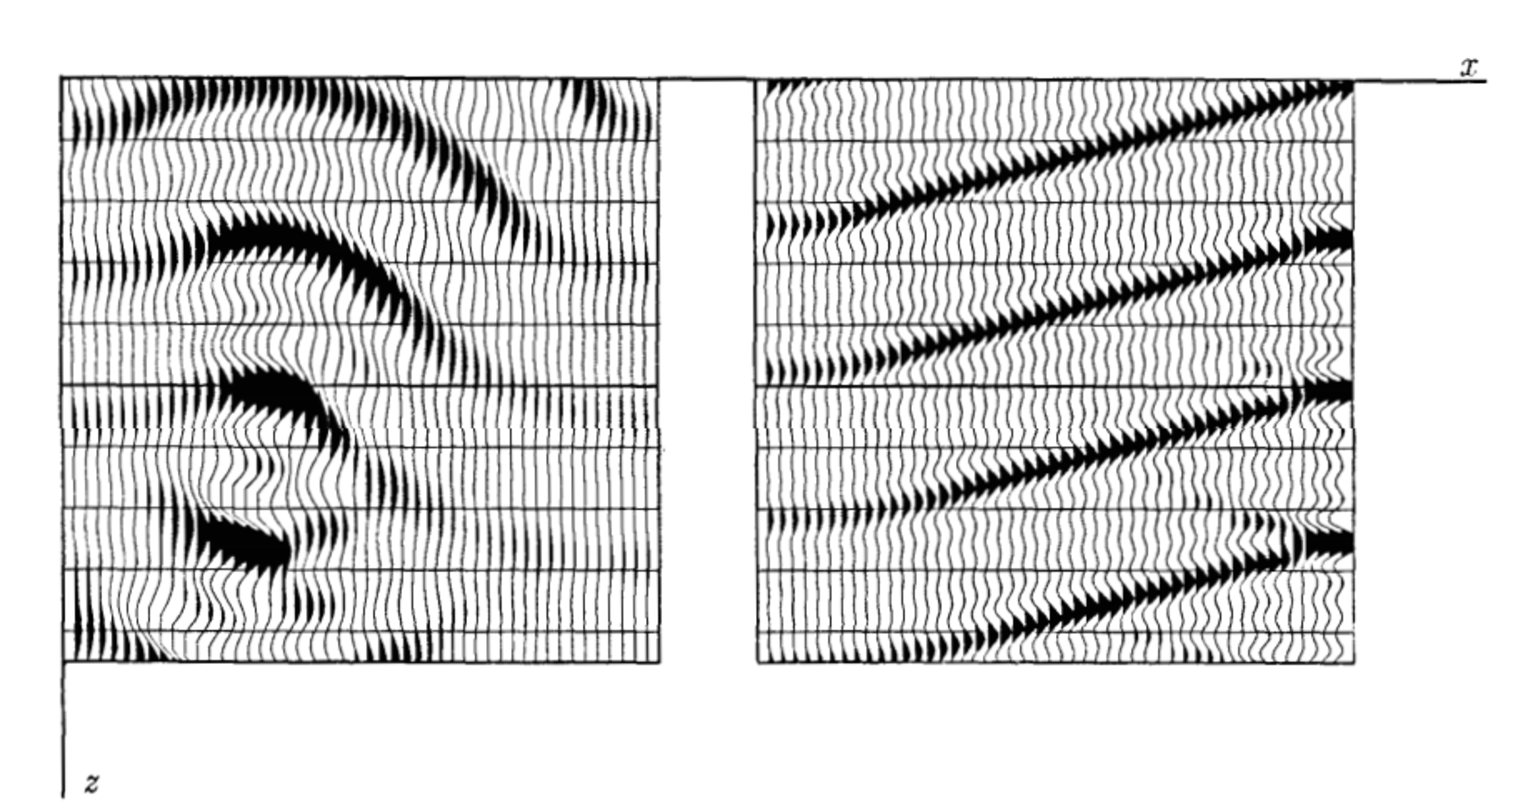
\includegraphics[width=0.85\textwidth]{new/fig-2-3-2}
\caption[2-3-2]{左:由图\ref{lst:code2.3.1}所产生的第一个电影画面;右:练习1的解}
\label{fig:new/fig-2-3-2}
\end{figure}

\begin{figure}[H]
\centering
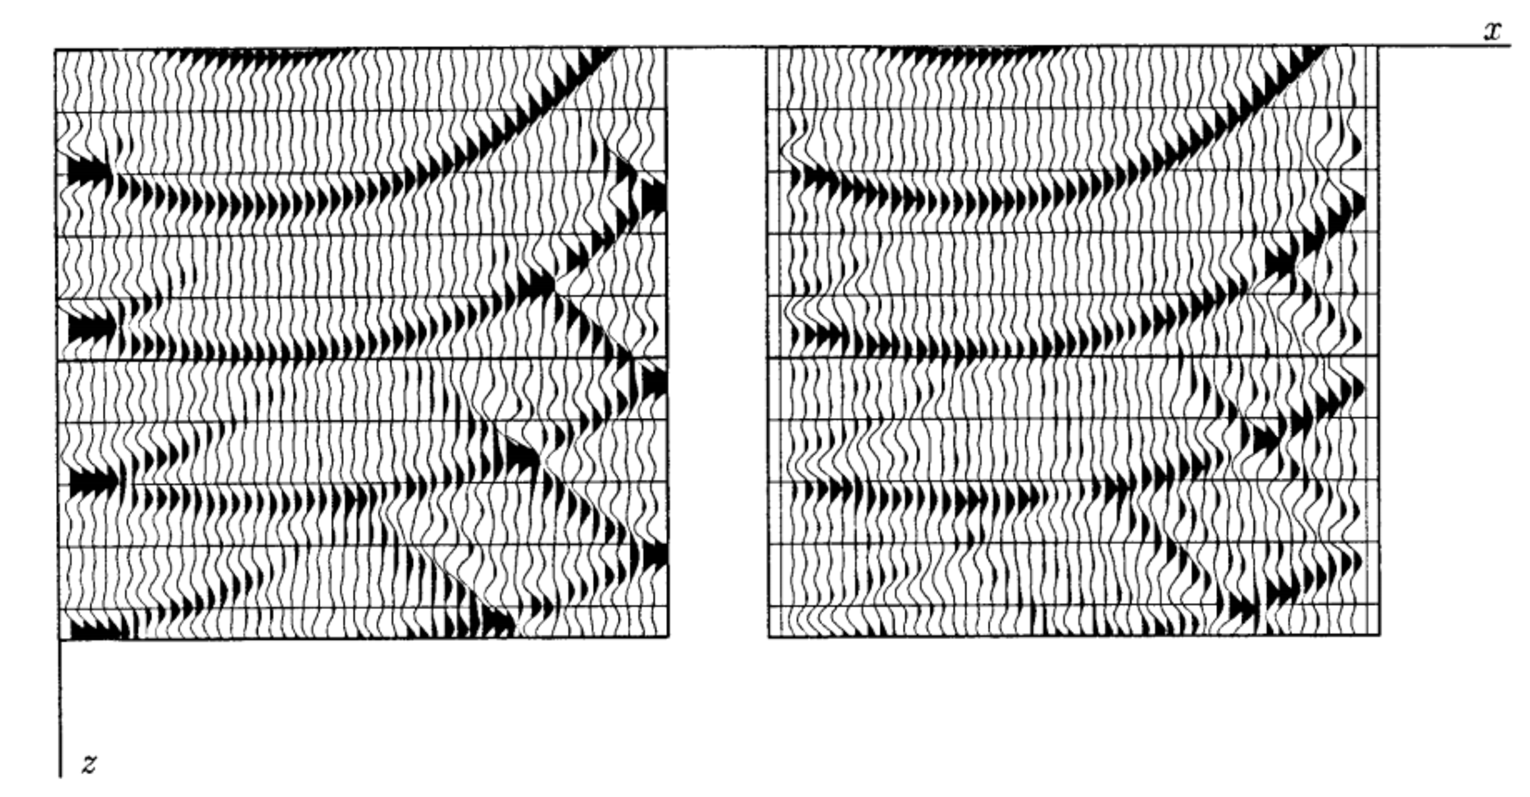
\includegraphics[width=0.85\textwidth]{new/fig-2-3-3}
\caption[2-3-3]{左:练习2,扩展的球面波;右:练习3,零值侧边界}
\label{fig:new/fig-2-3-3}
\end{figure}

\begin{figure}[H]
\centering
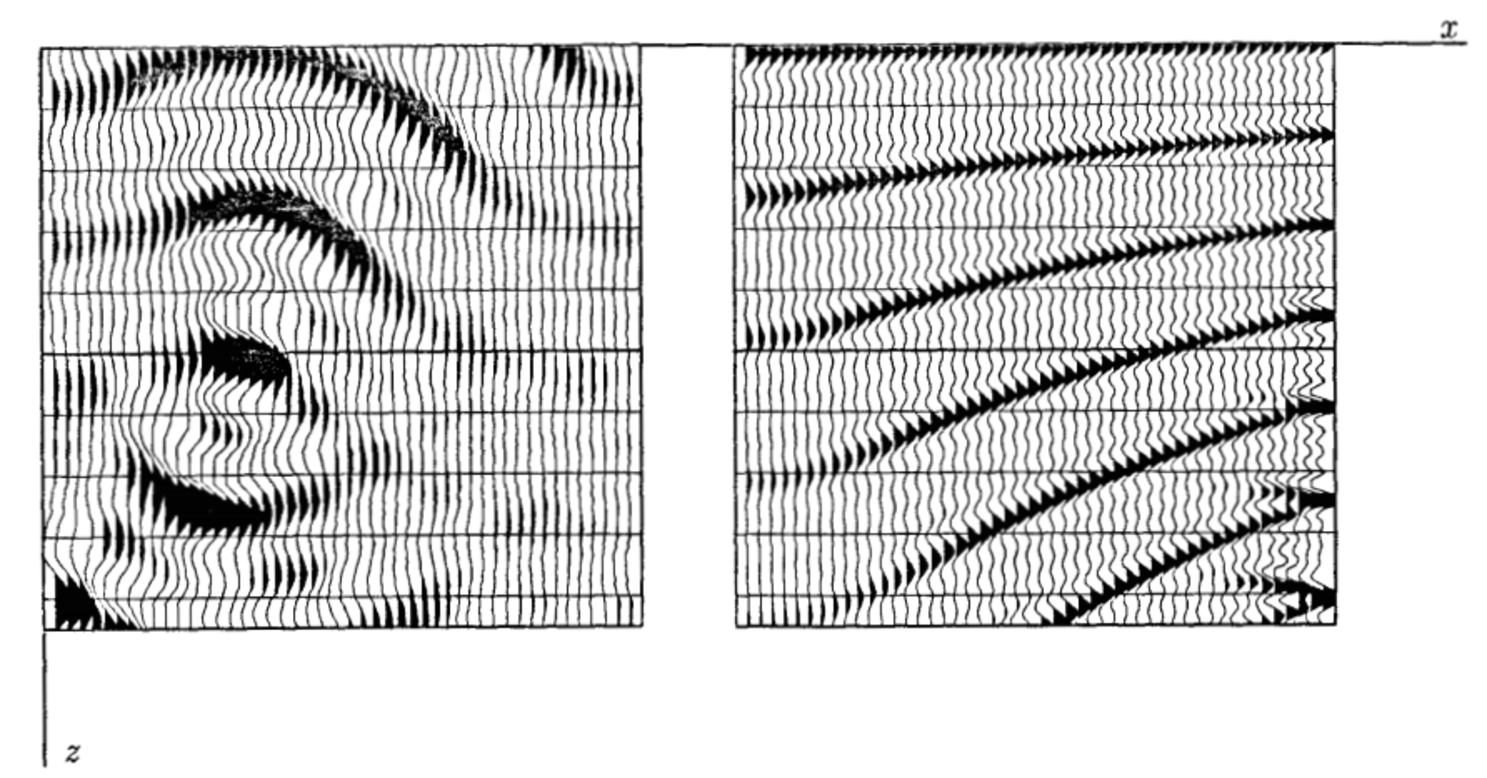
\includegraphics[width=0.85\textwidth]{new/fig-2-3-4}
\caption[2-3-4]{左:练习4,45°项;右:练习5,横向速度变化}
\label{fig:new/fig-2-3-4}
\end{figure}

\begin{figure}[H]
\centering
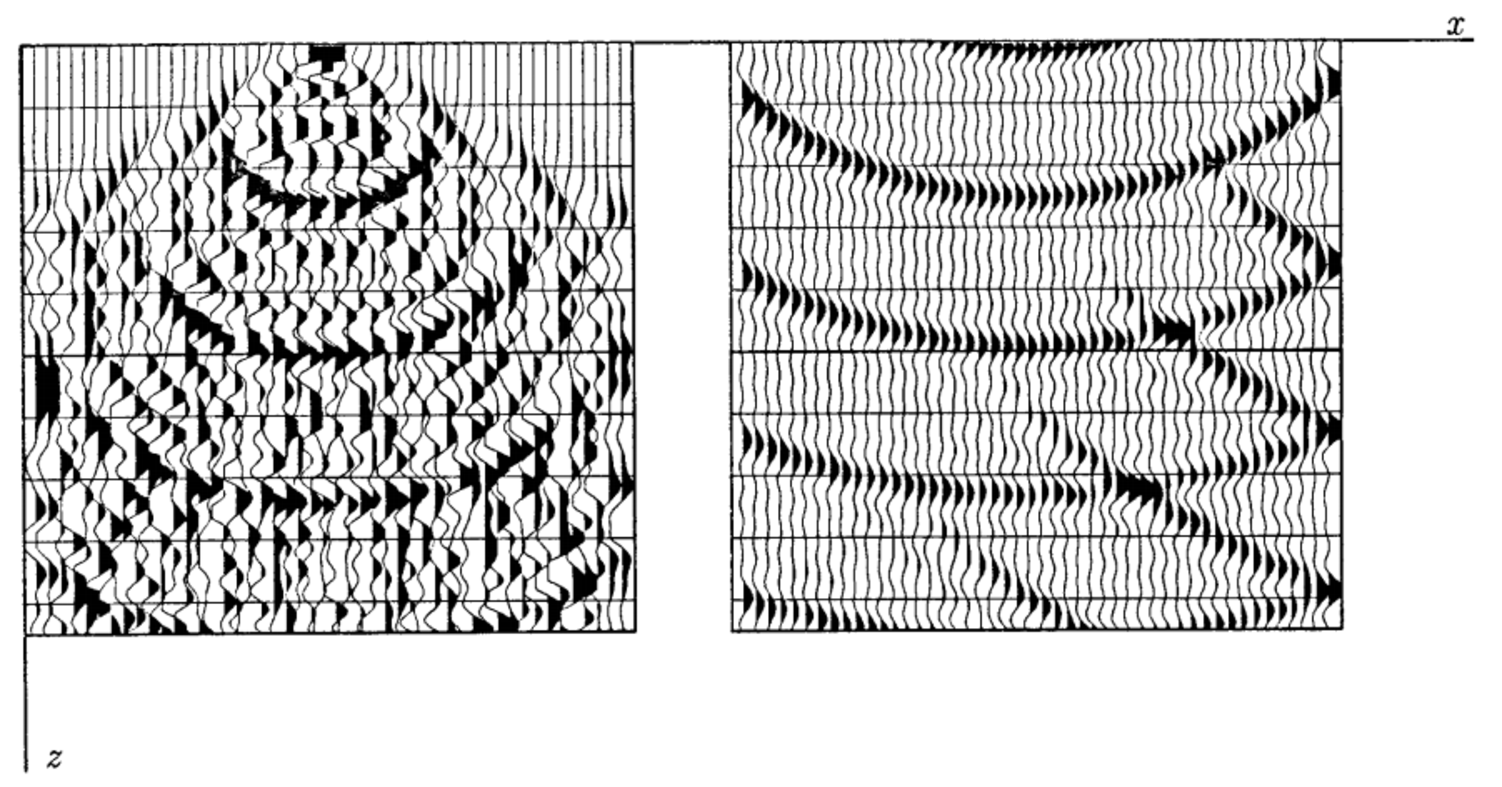
\includegraphics[width=0.85\textwidth]{new/fig-2-3-5}
\caption[2-3-5]{左:练习6,与点震源有关的计算假象;右:练习7,吸收边界}
\label{fig:new/fig-2-3-5}
\end{figure}

\begin{figure}[H]
\centering
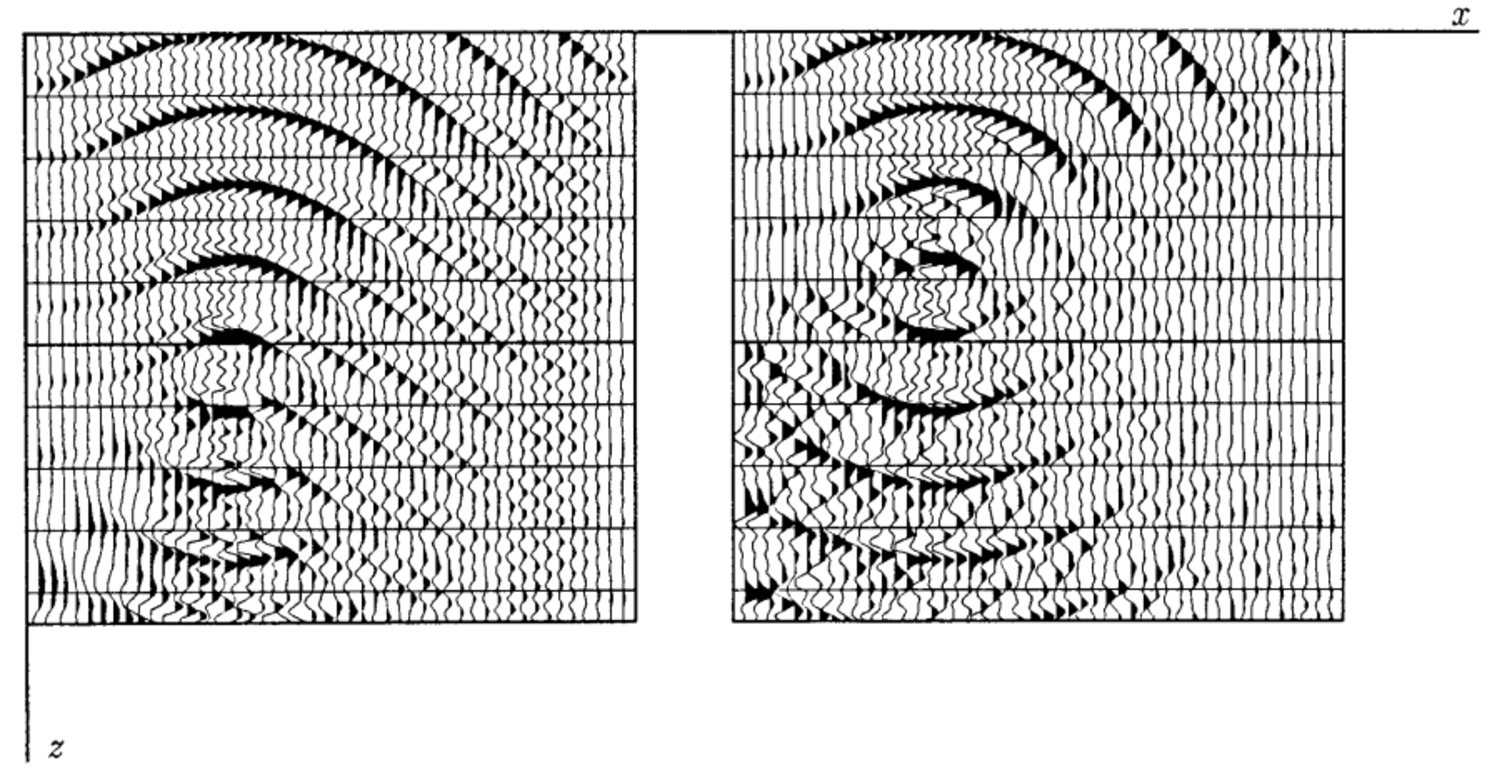
\includegraphics[width=0.85\textwidth]{new/fig-2-3-6}
\caption[2-3-6]{左:练习8,未采用1/6技巧;右:米用1/6技巧}
\label{fig:new/fig-2-3-6}
\end{figure}

\subsection{$(\omega,x,z)$域内的偏移程序(Kjartansson,Jacobs)}
偏移程序类似于循环影片程序,不过有一些差别。循环影片要作四重嵌套循环,它对时
间$t$的许多值产生结果。偏移则只要求在$t=0$时的值,所以省掉一重循环,这意味着用同等
数量的计算机时间可计算出更大的空间体积。可惜,失掉一次循环也就意味着失掉了以电
影形式显示的可能。采用$\omega$频率域偏移时,看来要考虑的唯一有意义的事就是输入与输出
了。

同循环电影不一样,这种过程的输入恐怕将会是野外数据了,所以不会存在频率域的解
析表达式。由于将在时间域内输入,因而必须进行Fourier变换。\ref{fig:new/2.3.7}所示程序的开始部
分定义一呰模拟野处数据的脉冲,这些全是宽脉冲,应将其偏移至近似半圆上。因为差分算子对微分算子的偏差会造成干扰混乱,所以就没利用准确的脉冲。

然后,该程序以Fourier变换方法把人工合成数据从时间域变换至频率域。

接着将每一频率成分向下延拓,这是沿深度$z$和沿频率$\omega$进行的一种循环。这两个循环
中随便那一个都可以是内循环,如何选择决定于计算机效率。

同循环影片程序要求用下行波方程不同,偏移是要求用上行波方程,所以要改变式
\ref{eq:ex2.3.1}中$z$轴的符号,这种改变影响到aa的符号和cshift的钼位符号。

和循环影片不同的另一个差别是,现在的输入有时间轴,而输出则仍为深度轴。习惯上为
方便起见,要重新组织计算过程,不是按深度而是按旅行时间“深度”显示,使输入与输出
的垂直轴相同。利用$\tau=z/v$与$d\tau/dz=1/v$的等价关系,由微分法则得出
\begin{equation}
\frac{\partial}{\partial z}=\frac{\partial\tau}{\partial z}\frac{\partial}{\partial \tau}=\frac{1}{v}\frac{\partial}{\partial \tau}
\label{eq:2.3.7}
\end{equation}
代入式(1)中,得
\begin{equation}
\frac{\partial P}{\partial \tau}= -i\omega P-\frac{v^2}{-i\omega 2}\frac{\partial^2 P}{\partial x^2}
\label{eq:2.3.8}
\end{equation}

在该程序中,时间采样间隔心=洫及旅行时间“深度”采样间隔$dtau=\Delta\tau$均取为1,因
此极大频率即是Nyquist频率。应注章,沿频率的循环只涉及正值频率轴。负值频率仅只用来保持时间函数为实函数,只需取实部就能很容易地做到这点。

% \begin{code}
% \begin{minted}[frame=single]{py}
% def my_func(x):
%     print x
% \end{minted}
% %\caption{My func}
% \label{lst:my_func}
% \end{code}
\begin{listing}[H]
  \caption{$(\omega,x,z)$域内的偏移程序}
  \inputminted{Fortran}{timespace/code2-3-7.f90}
  \label{lst:code2.3.7}
\end{listing}
偏移程序运算结果的输出如图\ref{fig:omx/kjartjac}所示。你看见的主要是半圆近似。在较晚的时间上
还有一些计算假象,可能是频率域假频影响所致。输入脉冲具有相当宽的倾斜条带状外形,
所以该图预告了以后将要加以证明的一件事实,即,半圆近似实际上是一个经过原点的椭
圆。

注意,原始脉冲的波形原是一种对称的时间函数,而现在半圆上的波形表现为既非对
称又非反对称,它是一种45°相移脉冲的波形,三维空间内一个点源所产生的波将具有90°相
移,由三维空间内一个二维爆炸反射面产生的波则应具有45°相移。

\begin{figure}[H]
\centering
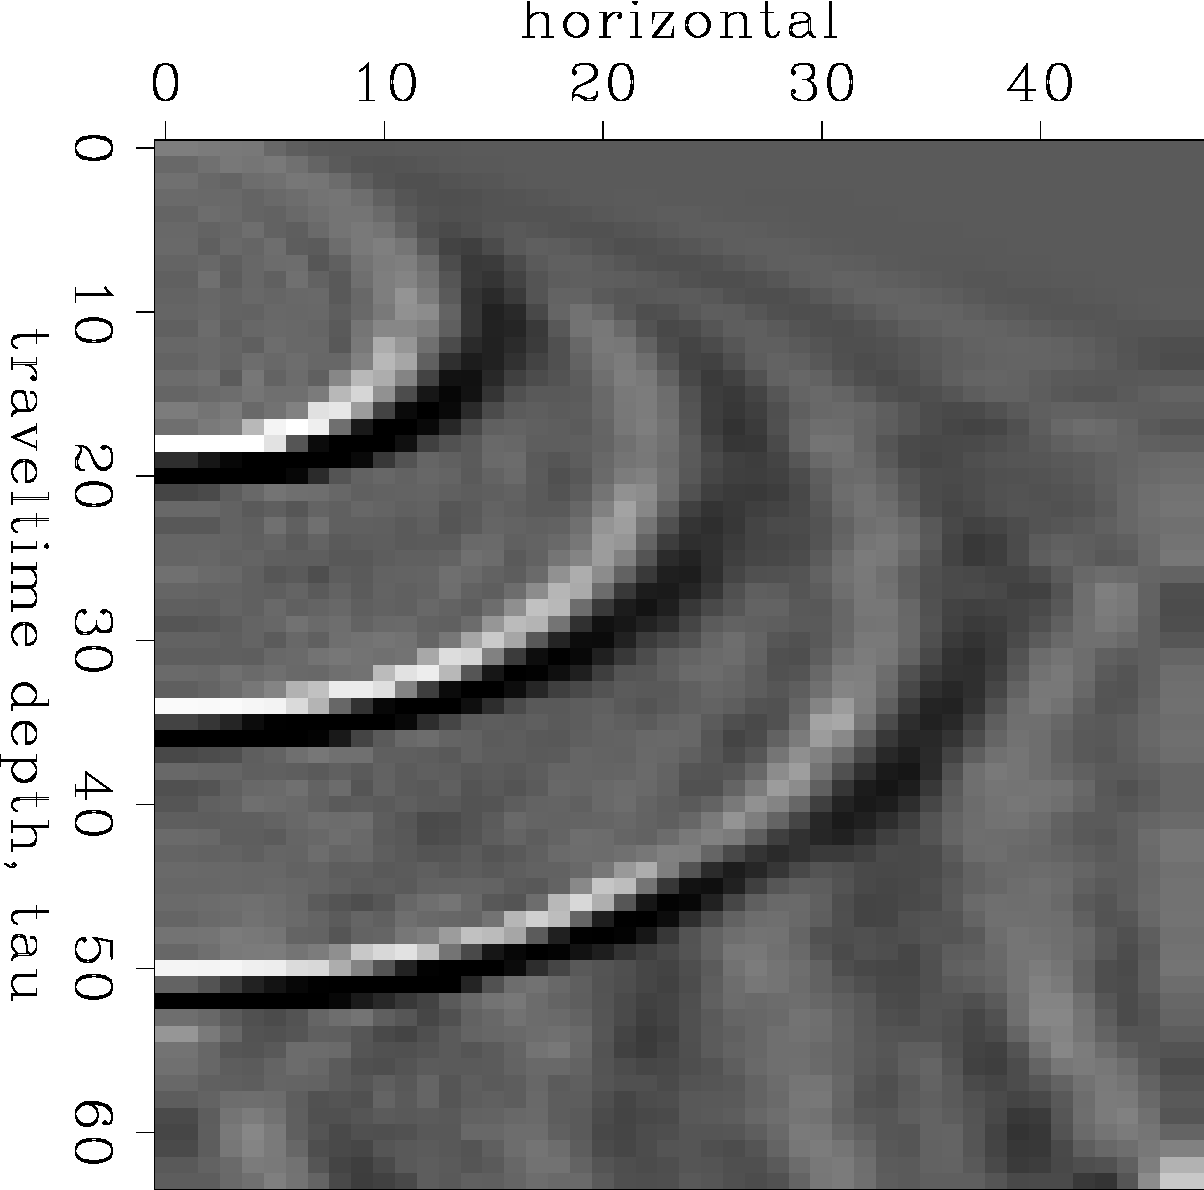
\includegraphics[width=0.5\textwidth]{omx/kjartjac}
\caption[kjartjac]{程序\ref{lst:code2.3.7}的输出:半圆近似}
\label{fig:omx/kjartjac}
\end{figure}
